\documentclass[oneside,a4paper,12pt]{report}
\usepackage[spanish]{babel}
\usepackage{hyphenat}
% support to write in spanish
\usepackage[utf8]{inputenc}
\usepackage{amsmath,amssymb}
\usepackage[]{amsthm}
\usepackage{lmodern}

% support to add non-formatted text
\usepackage{listings}

\usepackage{graphicx}
\usepackage{subfigure}
\usepackage{float}
\usepackage{epsfig}
\usepackage{epstopdf}
\usepackage{placeins}
\usepackage{acronym}

\usepackage{caption}
\usepackage[boxed]{algorithm2e}

\usepackage{tikz}
\usetikzlibrary{spy}

\hyphenation{or-de-na-mien-to}

% agregados por ccappo
\usepackage[toc,nomain,acronym,nonumberlist,nohypertypes=acronym,sort=def]{glossaries}
\usepackage{enumitem}

% -------------


\usepackage{array}
\usepackage[]{multirow}
\usepackage[]{multicol}
\usepackage[]{hhline}
\usepackage[final]{pdfpages}

\usepackage{caption}
\usepackage[boxed]{algorithm2e}

\newtheorem{theorem}{Teorema}
\newtheorem{proposition}{Proposition}
\newtheorem{lemma}{Lema}
\newtheorem{assumption}{Assumption}
\newtheorem{remark}{Remark}
\newtheorem{definition}{Definicin}


\SetKwInput{KwIn}{Entrada}
\SetKwInput{KwData}{Entrada}
\SetKwInput{KwResult}{Salida}
\SetKwInput{KwOut}{Salida}
\SetKwInput{Return}{retornar}
\SetKwFor{For}{desde}{hacer}{fin\_desde}
\SetKwFor{While}{mientras}{hacer}{fin\_mientras}
\SetKwIF{If}{ElseIf}{Else}{si}{entonces}{si\_no si}{si\_no}{fin\_si}


\graphicspath{{./structurePlot/}{./experiments/}{./bloques/}{./stagnation/}{./helmke/}{./Figures/}}
\DeclareGraphicsExtensions{{.eps}{.jpg}{.JPG}{.png}{.PNG}}

%%%%%%%%%%%%%%%%%%%%%%%%%%%%%%%%%%%%%%%%%%%%%%%%%%%%%%%%%%%%%%%%%%%%%%%%%%%%%%%%%%%%%%%%%%%%%%%%%%%
%\newglossary[symb]{symbol}{symb}{sym}{Lista de Smbolos}

%\addcontentsline{toc}{chapter}{Lista de Abreviaturas}
\chapter*{Lista de Abreviaturas}
%\myheader{LISTA DE ABREVIATURAS}
%\markboth{Lista de Abreviaturas}{Lista de Abreviaturas}

\hspace*{2em}
%Indice de abreviaturas
\acrodef{FHIR}{FHIR}
FHIR: Fast Healthcare Interoperability Resources.


%\input{symbols}

%\makeglossaries
%%%%%%%%%%%%%%%%%%%%%%%%%%%%%%%%%%%%%%%%%%%%%%%%%%%%%%%%%%%%%%%%%%%%%%%%%%%%%%%%%%%%%%%%%%%%%%%%%%%
\makeatletter
\newif\if@abstractmode

\renewenvironment{titlepage}
{
	\if@twocolumn
	\@restonecoltrue\onecolumn
	\else
	\@restonecolfalse\newpage
	\fi
	\if@abstractmode
	\thispagestyle{plain}%
	%\stepcounter{page}%
	\else
	\thispagestyle{plain}%
	%\setcounter{page}\@ne%
	\fi
}%
{\if@restonecol\twocolumn \else \newpage \fi
	\if@twoside\else
	\if@abstractmode
	\else
	\setcounter{page}\@ne%
	\fi
	\fi
}

\AtBeginEnvironment{abstract}{%
	\@abstractmodetrue%
}

%\makeatother

\makeatletter
\renewcommand{\maketitle}{\begin{titlepage}%
		%\null\vfil
		%\vskip 10\p@
		\thispagestyle{empty}
		\setcounter{page}{1}
		\noindent
		\begin{minipage}{0.3\textwidth}
			
\includegraphics[width=25mm]{./images/fpuna_logo_institucional.png}
		\end{minipage}
		\hfill%
		\begin{minipage}{0.7\textwidth}
			\raggedleft
			{\Large Universidad Nacional de Asunción}\\
			\vskip 1em%
			{\LARGE Facultad Politécnica}
		\end{minipage}

		\begin{center}
			\vskip 5em%
			{\large \@title \par}%
			\vskip 5em%
			{\large \@author }
			\vskip 1.5em%
			\vfill
			{\small \textit{Tesis presentada a la Facultad Politécnica, Universidad Nacional de Asunción, como requisito  para la obtención del Grado de Ingeniero en Informática.}}
			\vskip 1.5em%
			{San Lorenzo - Paraguay}  \\
			{Noviembre, 2019}
		\end{center}\par

		\newpage
		\noindent

		\begin{center}
			{\Large Universidad Nacional de Asunción}
			\vskip 1em
			{\LARGE Facultad Politécnica}
		\end{center}

		\begin{center}
			\vskip 5em%
			{\large \@title \par}%
			\vskip 5em%
			{\large \@author }
			\vskip 2.5em%
			\begin{tabular}[t]{cl}
				{\large Orientadores:}  \\
				& {\large Prof. Cynthia Villalba, Dr.} \\
				& {\large Prof. José Luis Vázquez Noguera, Dr.}
			\end{tabular}
			\vfill
			{\small \textit{Tesis presentada a la Facultad Politécnica, Universidad Nacional de Asunción, como requisito  para la obtención del Grado de Ingenierio en Informática.}}
			\vskip 1.5em%
			{San Lorenzo - Paraguay}  \\
			{Noviembre, 2019}
		\end{center}\par
	\end{titlepage}%
	\setcounter{footnote}{0}%
	\global\let\thanks\relax
	\global\let\maketitle\relax
	\global\let\@thanks\@empty
	\global\let\@author\@empty
	\global\let\@date\@empty
	\global\let\@title\@empty
	\global\let\title\relax
	\global\let\author\relax
	\global\let\date\relax
	\global\let\and\relax
}
\makeatother

\title{
	{\LARGE \textbf{Creación automática de arquetipo de integración de openEHR a partir de recurso de FHIR basado en equivalencias de tipos de datos}}
}

\author{\LARGE{Uriel Ivar González Benítez}}


%% Math Packages %%%%%%%%%%%%%%%%%%%%%%%%%%%%%%%%%%%%%%%%%%%%
%\usepackage{amsmath}
%\usepackage{amsthm}
%\usepackage{amsfonts}

%% Line Spacing %%%%%%%%%%%%%%%%%%%%%%%%%%%%%%%%%%%%%%%%%%%%%
\usepackage{setspace}
%\singlespacing        %% 1-spacing (default)
\onehalfspacing       %% 1,5-spacing
%\doublespacing        %% 2-spacing

%% Other Packages %%%%%%%%%%%%%%%%%%%%%%%%%%%%%%%%%%%%%%%%%%%
%\usepackage{a4wide} %%Smaller margins = more text per page.
%\usepackage{fancyhdr} %%Fancy headings
%\usepackage{longtable} %%For tables, that exceed one page


%%%%%%%%%%%%%%%%%%%%%%%%%%%%%%%%%%%%%%%%%%%%%%%%%%%%%%%%%%%%%
%% Remarks
%%%%%%%%%%%%%%%%%%%%%%%%%%%%%%%%%%%%%%%%%%%%%%%%%%%%%%%%%%%%%
%
% TODO:
% 1. Edit the used packages and their options (see above).
% 2. If you want, add a BibTeX-File to the project
%    (e.g., 'literature.bib').
% 3. Happy TeXing!
%
%%%%%%%%%%%%%%%%%%%%%%%%%%%%%%%%%%%%%%%%%%%%%%%%%%%%%%%%%%%%%

%%%%%%%%%%%%%%%%%%%%%%%%%%%%%%%%%%%%%%%%%%%%%%%%%%%%%%%%%%%%%
%% Options / Modifications
%%%%%%%%%%%%%%%%%%%%%%%%%%%%%%%%%%%%%%%%%%%%%%%%%%%%%%%%%%%%%

%\input{options} %You need a file 'options.tex' for this
%% ==> TeXnicCenter supplies some possible option files
%% ==> with its templates (File | New from Template...).

\setlength{\parindent}{1cm}
\usepackage{titlesec}

\fontsize{10pt}{12pt}\selectfont

\titleformat{\chapter}[display]
{\normalfont \sffamily%
	%\Huge% %change this size to your needs for the first line
	\fontsize{30pt}{25pt}\selectfont
	\bfseries}{\sffamily \chaptertitlename\ \thechapter}{20pt}{%
	\Huge %change this size to your needs for the second line
}

%\titleformat{\chapter}
%  {\normalfont\LARGE\bfseries}{\thechapter}{1em}{}

%%%%%%%%%%%%%%%%%%%%%%%%%%%%%%%%%%%%%%%%%%%%%%%%%%%%%%%%%%%%%
%% DOCUMENT
%%%%%%%%%%%%%%%%%%%%%%%%%%%%%%%%%%%%%%%%%%%%%%%%%%%%%%%%%%%%%
\setcounter{secnumdepth}{4}
\setcounter{tocdepth}{4}
\renewcommand{\listtablename}{ndice de Tablas}
\renewcommand{\tablename}{Tabla}
\renewcommand{\abstractname}{Resumen}
%\renewcommand{\algorithmname}{Algoritmo}
\SetAlgorithmName{Algoritmo}

% permite sacar la constante Capitulo de cada "chapter" y dejar
% numerado y con el ttulo de una seccion.
% --------------------------------------------
%\usepackage{titlesec}
%\titleformat{\chapter}
%  {\normalfont\LARGE\bfseries}{\thechapter}{1em}{}
%\titlespacing*{\chapter}{0pt}{3.5ex plus 1ex minus .2ex}{2.3ex plus .2ex}
% --------------------------------------------

% permite arreglar el problema de que las citas salen fuera del margen, hace

\usepackage{breakcites}

\begin{document}

\glsaddall % Colocar aqui para que funcione y agregue todos los acronimos aun si no se especificaron con \gls.

\pagenumbering{roman}

\maketitle

\newcolumntype{C}[1]{>{\centering\arraybackslash}m{#1}}

\clearpage

\renewcommand{\abstractname}{{\normalfont Hoja de Aprobación de Tesis}}
\abstract{
	\setcounter{page}{3}

	\vspace{+10pt}

	\begin{center}
		{\Large \textbf{Creación automática de arquetipo de integración de openEHR a partir de recurso de FHIR basado en equivalencias de tipos de datos}}
	\end{center}
	\

	\begin{center}
		\textbf{Uriel Ivar González Benítez}
	\end{center}

	\vspace{+20pt}

	\begin{flushleft}
		Tesis de Grado aprobada el XX de Noviembre de 2019 por los siguientes miembros del Jurado de Defensa:
	\end{flushleft}

	\vspace{+20pt}

	\begin{tabular}{rr}
		& Prof. Dr. Cynthia Villalba (FP-UNA), orientador \\
		& Prof. Dr. José Luis Vázquez Noguera (FP-UNA), co-orientador \\
	\end{tabular}

	\vspace{+90pt}

	\noindent
	\begin{tabular}{cC{0.6cm}c}
		\textbf{Prof. Dr. Cynthia Villalba} & &\textbf{Prof. Dr. José L. Vázquez N.} \\
		Orientador & &Co-Orientador \\
	\end{tabular}

}


% \newcommand{\myalfnt}[1]{\small #1}
% \SetAlFnt{\myalfnt}

\renewcommand\figurename{Figura}
\renewcommand\tablename{Tabla}
\renewcommand\partname{Parte}
\renewcommand\chaptername{Captulo}
\renewcommand\appendixname{APENDICE}
\renewcommand\abstractname{RESUMEN}
\renewcommand\proofname{Demostracin}
% \renewcommand\algorithmname{Algoritmo}



%\renewcommand\fcontentsname{NDICE GENERAL}
%\renewcommand\listfigurename{LISTA DE FIGURAS}
%\renewcommand\listtablename{LISTA DE TABLAS}
%\renewcommand\bibname{REFERENCIAS BIBLIOGRFICAS}
%\renewcommand\indexname{LISTA DE SMBOLOS}

\SetAlgorithmName{Algoritmo}{algoritmo}{LISTA DE ALGORITMOS}



    \renewcommand{\abstractname}{}
  \abstract{
  	\thispagestyle{empty}
  	\begin{flushright}
	  	\textit{Dedicación en progreso...\\
		\textbf{Uriel González}}
  	\end{flushright}

  }

    \renewcommand{\abstractname}{{\sffamily \large Agradecimientos}}
  \abstract{
En progreso...

	\begin{flushright}
  	\textbf{Uriel González}
	\end{flushright}

  }

  \renewcommand{\abstractname}{}
\abstract{
	\vspace{-20pt}
   \begin{center}
	\textbf{Creación automática de arquetipo de integración de openEHR a partir de recurso de FHIR basado en equivalencias de tipos de datos} \\
	\textsl{Autor}: Uriel Ivar González Benítez
   \end{center}

\indent \textit{Orientadores:} \\
\indent \indent Prof. Dr. Cynthia Villalba. \\
\indent \indent Prof. Dr. José Luis Vázquez Noguera. \\

{\sffamily \large \textbf{Resumen}}

En progreso...

{
	\par\vfill
    \noindent\textbf{Palabras clave:} Interoperabilidad; FHIR; openEHR; arquetipo de integración.
}


}

    \renewcommand{\abstractname}{}
  \abstract{
  	\begin{center}
  		\vspace{-20pt}
  		\textbf{Automatic creation of openEHR integration archetype from FHIR resource based on equivalencies in data types} \\
  		\indent \textsl{Author}: Uriel Ivar González Benítez \\
  	\end{center}

  	\indent \textit{Advisors:} \\
  	\indent \indent Prof. Dr. Cynthia Villalba. \\
	\indent \indent Prof. MSc. José Luis Vázquez Noguera. \\

  	{\sffamily \large \textbf{Summary}}

  	%\begin{foreignabstract}

In progress ...

  	{%
  		\par\vfill
  	\noindent\textbf{Keywords:} interoperability; FHIR; openEHR; integration archetype.
    }
  }



  \renewcommand{\contentsname}{Apndice General}
  \renewcommand{\bibname}{Referencias Bibliogrficas}
  \renewcommand{\listtablename}{Lista de Tablas}
  \renewcommand{\listfigurename}{Lista de Figuras}
  \renewcommand{\listalgorithmcfname}{Lista de Algoritmos}  % agregar al TOC la lista de Algoritmos

  \tableofcontents

  \cleardoublepage
  \addcontentsline{toc}{chapter}{\listfigurename}  % agregar al TOC la lista de figuras
  \listoffigures

  \addcontentsline{toc}{chapter}{\listtablename} % agregar al TOC la lista de tablas
  \listoftables
  \addcontentsline{toc}{chapter}{Lista de Abreviaturas}
\chapter*{Lista de Abreviaturas}
%\myheader{LISTA DE ABREVIATURAS}
%\markboth{Lista de Abreviaturas}{Lista de Abreviaturas}

\hspace*{2em}
%Indice de abreviaturas
\acrodef{FHIR}{FHIR}
FHIR: Fast Healthcare Interoperability Resources.

  %\setlist[description]{leftmargin=!, labelwidth=5em} % alinear la descripcion

  %%%%%%%%%%%%%%%%%%%%%%%%%%%%%%%%%%%%%%%%%%%%%%%%%%%%%%%%%%%%%%%%%%%%%%%%%%%%%%%%%%%%%%%%%%%%%%%%%%%%%%
  %\printglossary[type=\acronymtype, title=Lista de Abreviaciones, toctitle=Lista de Abreviaciones]
  %\printglossary[type=symbol,title=Lista de Smbolos, toctitle=Lista de Smbolos]
  %%%%%%%%%%%%%%%%%%%%%%%%%%%%%%%%%%%%%%%%%%%%%%%%%%%%%%%%%%%%%%%%%%%%%%%%%%%%%%%%%%%%%%%%%%%%%%%%%%%%%%
  %\setlist[description]{style=standard} % volver a colocar en su formato original
 \clearpage
 \pagenumbering{arabic}

  %\mainmatter
    \chapter{Introducción}

La coordinación asistencial involucra compartir información entre todos los actores interesados en el cuidado del paciente para lograr una mejor atención \cite{CareCoordination}. Sin embargo, esta información se encuentra dispersa entre diferentes sitios, dificultando la continuidad asistencial \cite{Indarte11}.

Un factor crucial para una adecuada continuidad de cuidados es la interoperabilidad de los sistemas de información que dan soporte al proceso asistencial por medio de estándares \cite{OPS16}. Para garantizar que la información intercambiada entre sistemas de información de salud pueda ser entendida correctamente, procesada y utilizada de forma efectiva se debe estandarizar conceptos clínicos y otros conceptos de dominio usando terminologías (LOINC, SNOMED-CT, UCM, etc.) \cite{ISO20514}.

En el ámbito de la salud, uno de los estándares más prometedores es Fast Healthcare Interoperability Resources (FHIR) desarrollado por Health Level 7 (HL7). FHIR combina las funcionalidades de HL7 v2, v3 y CDA con los estándares web (XML, JSON, HTTP, OAuth, etc.) \cite{FHIR}. FHIR se basa en recursos que son los componentes básicos para todos los intercambios. Los recursos describen información clínica y administrativa. Además de definir los recursos, FHIR especifica un conjunto de interfaces, las cuales son usadas por los sistemas para compartir información. Otro estándar de amplio uso es openEHR publicado por openEHR Foundation. OpenEHR especifica una plataforma para construir sistemas EHR \cite{openEHR}. OpenEHR se basa en el modelado de dos niveles que distingue un modelo de referencia y arquetipos \cite{Bale00}. El modelo de referencia es un modelo de información estable que define las estructuras lógicas de los EHR. Los arquetipos son las definiciones formales de conceptos clínicos construidos sobre el modelo de referencia. Uno de los propósitos de los arquetipos es el de garantizar la interoperabilidad.

Algunos sistemas de salud buscan compartir información a través de repositorios de datos openEHR por medio de interfaces FHIR \cite{Lopez16}. Para ello, se necesita encontrar equivalencias entre los datos que se comparten - recursos FHIR - y el modelo de dominio de los repositorios de datos - arquetipos openEHR-. Dichas equivalencias posibilitarán, a partir de instancias de recursos FHIR, generar datos en repositorios openEHR y viceversa.

El objetivo de este trabajo es describir un proceso automatizado para crear arquetipos de integración openEHR a partir de definiciones de recursos FHIR utilizando equivalencias entre los tipos de datos de openEHR y FHIR. Estas equivalencias se encuentra de manera manual siguiendo la metodología presentada como parte del trabajo. Los arquetipos de integración creados ayudarán a intercambiar los datos entre instancias de arquetipos openEHR e instancias de recursos FHIR. El resto de este trabajo está organizado en 4 secciones. Sección 2 presenta las principales características de FHIR y openEHR, y la arquitectura de conversión de datos modelo. Sección 3 describe la creación de arquetipos de integración openEHR de recursos FHIR utilizando la metodología propuesta. Sección 4 muestra las equivalencias entre los tipos datos FHIR y openEHR, un arquetipo de integración openEHR creado con la metodología propuesta, y la comparación entre la creación automática y la manual. Finalmente, Sección 5 presenta las conclusiones del trabajo.

    \chapter{Antecedentes}

FHIR (Fast Health Interoperability Resources) es un estándar para intercambiar información del cuidado de la salud electrónicamente \cite{FHIRClinician}. FHIR ofrece un fuerte enfoque en la implementabilidad en una amplia variedad de arquitecturas y escenarios \cite{FHIRExecutive}. La versión actual de FHIR se publica como un estándar para uso experimental \cite{FHIR}.

OpenEHR es un enfoque de plataforma para el desarrollo de soluciones de tecnología de la información para el cuidado de la salud. OpenEHR provee un conjunto de estándares para modelos de información clínica, extractos de EHR, datos demográficos, tipos de datos y varios tipos de interfaces de servicio \cite{openEHRWhitePaper}.

\section{FHIR}

FHIR define recursos para representar conceptos administrativos tales como paciente, proveedor, organización y dispositivo, así como conceptos clínicos que cubren problemas, medicamentos, diagnósticos, planes de atención y más \cite{FHIRResourceList}.

Los recursos tienen en común las siguientes características \cite{FHIRDeveloper}:
\begin{itemize}
  \item una URL que identifica el recurso;
  \item una metainformación común;
  \item un texto legible por el ser humano para la seguridad clínica;
  \item un conjunto definido de elementos de datos diferente para cada recurso;
  \item un marco para extender y adaptar los recursos existentes.
\end{itemize}

Los recursos se describen usando recursos StructureDefinition \cite{FHIRStructureDefinition}. Estos recursos StructureDefinition definen un conjunto de elementos de datos. Cada elemento incluye una ruta, una cardinalidad y un tipo de dato \cite{FHIRElementDefinition}.

La ruta del elemento de dato es la propiedad más importante de la definición del elemento. Esta ruta localiza el elemento en una jerarquía definida dentro del recurso \cite{FHIRElementDefinition}.

El tipo de dato del elemento de dato puede ser primitivo o complejo \cite{FHIRDataTypes}. La diferencia entre ambos tipos de datos es que el primitivo permite un solo valor para el elemento,  mientras que el complejo puede tener elementos hijos. Cada tipo de dato primitivo es una 3-tupla, que consiste en a) un dominio de valores, que incluye la definición del tipo de dato, b) una representación XML y c) una representación JSON. Dentro de los tipos de datos complejos se encuentran: los de propósito general, los tipos para metadatos y los de propósito especial.

Cada elemento de dato puede ser extendido o restringido \cite{FHIRProfiling}. El elemento de dato se extiende para representar información adicional que no forma parte de la definición del recurso\cite{FHIRExtensibility}. Cada recurso solo incluye elementos de datos si la mayoría de las implementaciones usarán esos elementos de datos en particular \cite{FHIRArchitecture}. El elemento de dato se restringe cambiando su cardinalidad.

Los recursos soportan la vinculación a terminología clínica, lo cual contribuye a lograr la interoperabilidad semántica \cite{FHIRArchitecture}.

Aparte de las definiciones de los recursos, FHIR define un conjunto de interfaces por las cuales los sistemas comparten los recursos. Los mecanismos de intercambio soportados son los siguientes \cite{FHIRClinician}:
\begin{itemize}
  \item a través de una interfaz REST;
  \item mediante el intercambio de documentos;
  \item vía el envío y recepción de mensajes;
  \item la exposición e invocación de servicios.
\end{itemize}

\section{OpenEHR}

El enfoque de openEHR es un riguroso modelado del conocimiento, y se basa en el principio básico de separación de los dominios de concepto y los dominios de información en los sistemas de información. Los dominios de concepto son modelados usando los arquetipos y expresados en el Lenguaje de Definición de Arquetipos (ADL).

\subsection{Modelado en openEHR}

El enfoque de openEHR para el modelado es multinivel. Los modelos son desarrollados y mantenidos por expertos de dominio en su propio nivel \cite{openEHRArchitecture}.

El primer nivel se basa en el modelo de referencia. El modelo de referencia corresponde al modelo de información estable, por ejemplo, tipos de datos o estructuras de datos. Todos los datos EHR en cualquier sistema openEHR obedecen el modelo de referencia. Solo este primer nivel es implementado en software \cite{openEHRArchitecture}.

El siguiente nivel consiste en los arquetipos. Los arquetipos corresponden a los contenidos del dominio, por ejemplo, medidas de la presión sanguínea o resultado de la prueba para diabetes. Estos arquetipos son modelados por profesionales clínicos o expertos en informática de la salud sin ningún conocimiento tecnológico de los sistemas finales. Los arquetipos son almacenados en sus propios repositorios.

Las plantillas constituyen el siguiente nivel. Estas plantillas especifican grupos de arquetipos que se usan para un propósito particular, y a menudo corresponden a formularios de pantalla \cite{openEHRArchitecture}.

En el último nivel se encuentran los artefactos generados a partir de las plantillas \cite{openEHR}. Los artefactos, mostrados en la Figura \ref{fig:openeEHR_ecosystem}, no se modelan manualmente. Esto significa que un modelo para resultado de microbiología solo necesita hacerse una vez para habilitar los informes, formularios de interfaz de usuario, documentos y otros formatos de mensaje que se generarán.

\begin{figure}[h]
  \centering
  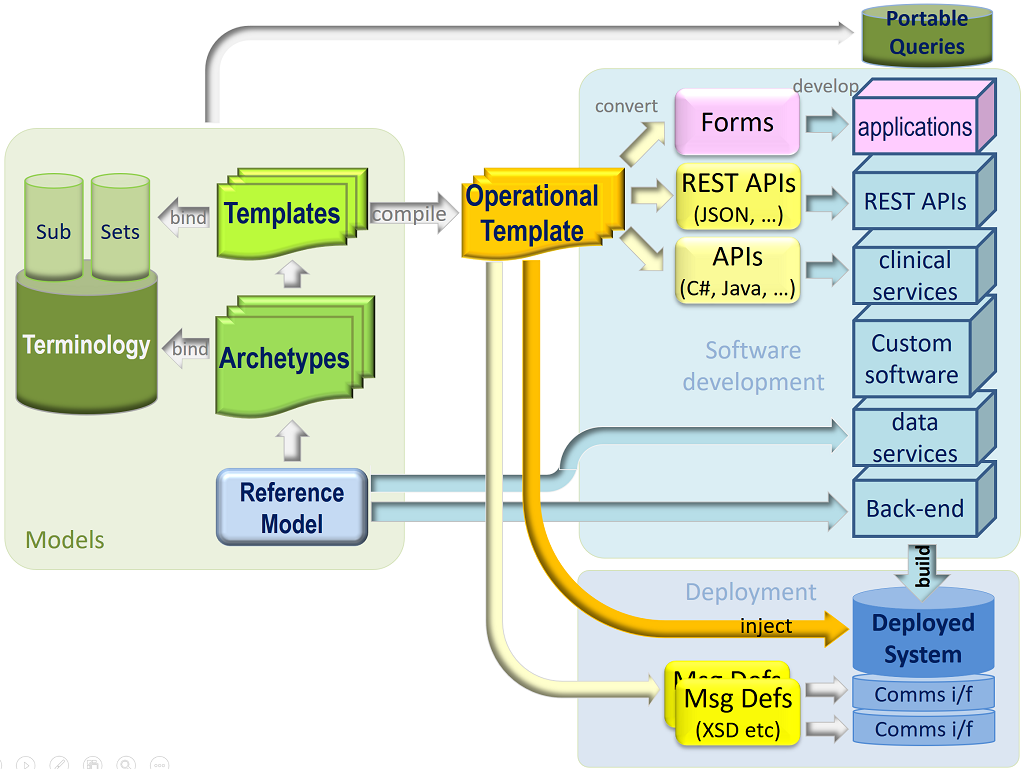
\includegraphics[scale=0.6]{./images/openehr_dev_ecosystem.png}
  \caption{Enfoque openEHR (Fuente: Extraído desde \cite{openEHR}).}
  \label{fig:openeEHR_ecosystem}
\end{figure}

\subsection{Arquetipos}

Cada arquetipo es un conjunto de restricciones en el modelo de referencia, definiendo un contenido de dominio \cite{openEHRArchitecture}. Las restricciones definen configuraciones de instancias del modelo de referencia consideradas conformes al arquetipo. Por ejemplo, ciertas configuraciones de las clases PARTY, ADDRESS, CLUSTER y ELEMENT pueden definirse por un arquetipo Person como estructuras permitidas para personas con identidad, contactos y direcciones \cite{openEHRAOM}.

Los arquetipos pueden tener relaciones de especialización o composición. Los arquetipos especializados son creados restringiendo aún más las restricciones existentes de otros arquetipos. Los arquetipos compuestos son definidos a partir de otros arquetipos \cite{openEHRArchitecture}.

OpenEHR incluye un mecanismo de rutas. Estas rutas pueden usarse para referenciar a cualquier dato dentro de un arquetipo \cite{openEHRArchitecture}.

Los arquetipos proveen una forma de definir el significado de los datos, y de conectar los datos a terminologías conocidas como SNOMED CT, LOINC, ICPC, ICDx y muchas otras terminologías y vocabularios usados en salud \cite{openEHRArchitecture}.

\subsection{Lenguaje de Definición de Arquetipo}

Los arquetipos son expresados en el Lenguaje de Definición de Arquetipo \cite{openEHRADL} (ADL por sus siglas en inglés). ADL utiliza tres sintaxis: cADL (forma de restricción de ADL), ODIN (notación de instancia de datos de objeto) y una versión de lógica de predicado de primer orden (FOPL por sus siglas en inglés).

Las restricciones de cADL se escriben en un estilo estructurado en bloques, similar a los lenguajes de programación estructurados en bloques como C. Cada bloque se introduce mediante un identificador de un modelo de información de openEHR. Los identificadores alternan entre los nombres de tipo conocidos como bloques de objetos o nodos de objeto y los nombres de atributos de tipo conocidos como bloques de atributo o nodos de atributos. El uso de nodos de objeto permite la formación de rutas de arquetipo, que se pueden utilizar para hacer de forma inequívoca a nodos de objetos dentro del mismo arquetipo \cite{openEHRADL}.

La sintaxis de cADL se utiliza para expresar la definición de los arquetipos, mientras que la sintaxis de ODIN se usa para expresar datos que aparecen en las secciones de idioma, descripción, terminología y revisión histórica de un arquetipo.

Actualmente hay dos versiones principales existentes: `ADL 1.4', la versión original, y `ADL 2', una versión más moderna, que se está adoptando lentamente.

\section{Arquitectura de conversión de datos}

La arquitectura del Modelo de Información de Integración de openEHR, mostrada en la Figura \ref{fig:data_conversion_architecture}, está diseñada para situaciones de integración heredadas.

\begin{figure}[h]
  \centering
  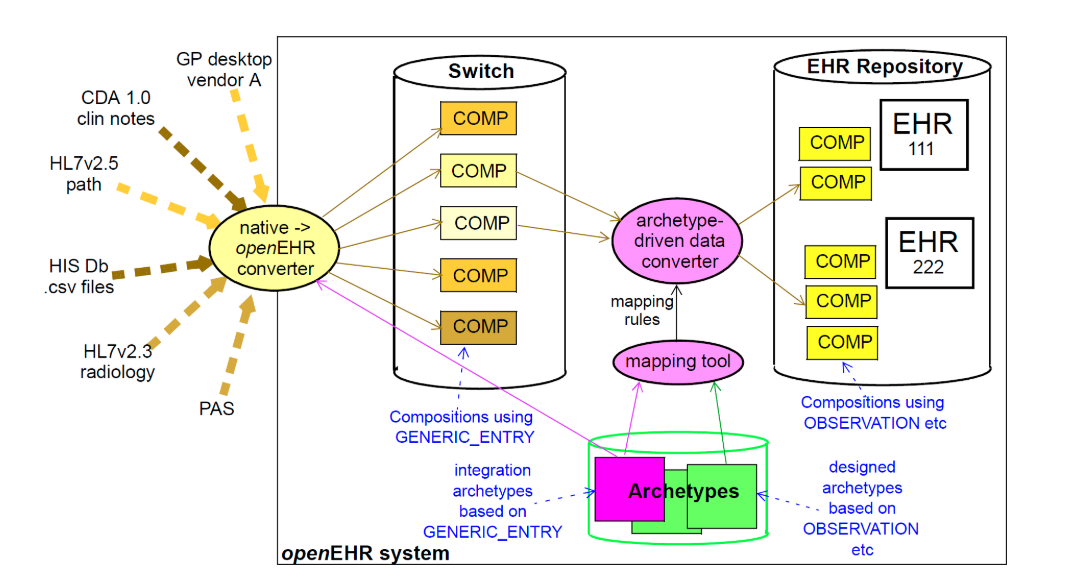
\includegraphics[scale=0.4]{./images/data_conversion_architecture.png}
  \caption{Integración de dato dentro de openEHR (Fuente: Extraído desde \cite{openEHR}).}
  \label{fig:data_conversion_architecture}
\end{figure}

El diseño se basa en una clara separación de la transformación sintáctica y semántica requerida en los datos importados en openEHR. La transformación sintáctica convierte los datos de su formato sintáctico original en estructuras del modelo de referencia de openEHR, cuya estructura lógica y semántica está controladas por arquetipos de integración que imitan el diseño original de los datos. Como resultado de la conversión, los datos pueden ser procesados en openEHR. La transformación semántica convierte los datos importados a arquetipos clínicos.

Los elementos de openEHR que hacen posible esta transformación son:
\begin{itemize}
  \item la clase GENERIC\_ENTRY que se utiliza para crear representaciones intermedias de datos de fuentes que de otra manera no se ajustan a las clases openEHR;
  \item arquetipos de integración definidos a partir de la clase GENERIC\_ENTRY;
  \item arquetipos clínicos diseñados a partir de las subclases de ENTRY;
  \item reglas de transformación semántica entre arquetipos de integración y arquetipos clínicos.
\end{itemize}

FHIR y openEHR comparten cierta similitud. Los recursos de FHIR y los arquetipos de openEHR definen patrones reutilizables para la descripción precisa de la información clínica \cite{Bosca15}. Sin embargo, los trabajos de colaboración entre las comunidades de FHIR y openEHR \cite{Collaboration} no consiguieron generar recursos y arquetipos con un contenido coincidente y clínicamente verificable. Una de las causas son los principios de diseño diferentes utilizados por ambas comunidades. Siendo la principal diferencia que los arquetipos esperan representar la mayoría del contenido clínico, mientras que los recursos solo contienen la información clínica utilizada más común.

El enfoque propuesto en este trabajo utiliza los recursos FHIR StructureDefinition para crear arquetipos de integración de openEHR usando las clases CLUSTER y ELEMENT. Estos arquetipos de integración, expresados en ADL, facilitarán el intercambio de datos entre sistemas FHIR y sistemas openEHR. El intercambio se logra estableciendo mapeos entre las rutas de los elementos de los recursos y las rutas de los nodos de los arquetipos. A diferencia de la clase GENERIC\_ENTRY que no hace suposiciones sobre la forma real de los datos, las clases CLUSTER y ELEMENT representan la estructura jerárquica de los recursos FHIR. Además, el enfoque propuesto hace uso de vinculaciones, conexiones entre modelos de información y terminologías, soportados por ambos estándares para conservar el significado de los datos intercambiados.

    \chapter{Método Propuesto}

Una forma de establecer equivalencias entre un recurso FHIR y un arquetipo de integración openEHR es identificando relaciones entre elementos de datos del recurso FHIR y restricciones del arquetipo de integración openEHR. Para ello se crea un arquetipo de integración openEHR a partir de la definición del recurso FHIR existente.

La creación del arquetipo de integración openEHR a partir de la definición del recurso FHIR utilizando equivalencias entre tipos de datos puede ser sencilla. El arquetipo de integración openEHR se puede crear de forma manual dentro de un editor de arquetipos como los citados en \cite{openEHRModellingTools}. Este se modela con la misma estructura del recurso FHIR. Cada tipo de dato de FHIR de la estructura se sustituye por su equivalente tipo de dato de openEHR. En este trabajo, se presenta una alternativa diferente consistente en la creación a través de un proceso automatizado. Las ventajas de la creación automática son tiempo de creación y riesgo de introducir errores por factor humano menores a los de la creación manual.

\section{Equivalencias entre tipos de datos}

La definición de un elemento en un recurso FHIR incluye tipo de dato \cite{FHIRElement}. Por lo tanto, un prerequisito es encontrar equivalencias entre tipos de datos FHIR y tipos de datos openEHR. Las equivalencias permitirán crear arquetipos openEHR a partir de definiciones de recursos FHIR.

Dada la función \( f(x) \) que retorna el dominio de valores que se le puede asignar a un dato \( x \), \( A \) el conjunto de atributos del tipo de dato de openEHR \( o \), la equivalencia entre el tipo de dato de FHIR \( p \)  y el tipo de dato de openEHR \( o \) existe si se cumplen las condiciones de:

\begin{enumerate}
  \item \( \exists a \in A \land f(a) \supseteq f(p) \);
  \item los propósitos de \( o \) y \( p \) son similares.
\end{enumerate}

Las equivalencias se encuentran al realizar una revisión manual exhaustiva del conjunto de tipos de datos de FHIR \cite{FHIRDataTypes} y del Modelo de Información de Tipos de Datos de openEHR \cite{openEHRDataTypes}. En primer lugar, para cada tipo de dato de FHIR se agrupa los tipos de datos de openEHR que tengan algún atributo cuyo dominio de valores sea un superconjunto del dominio de valores del tipo de dato de FHIR. Posteriormente, se analiza y compara las definiciones, incluyendo el propósito, de cada tipo de dato de FHIR y su grupo de tipos de datos de openEHR encontrados inicialmente. Solo para el tipo de FHIR boolean se utiliza la definición de \cite{W3C} por no tener una definición explícita en la especificación de FHIR y por ser un tipo de dato importado desde W3C.

Como ejemplo, el tipo de FHIR boolean y el tipo de openEHR DV\_BOOLEAN reúnen ambas condiciones, por lo tanto, son equivalentes:
\begin{enumerate}
  \item los valores true y false del dominio de valores del tipo boolean pueden ser almacenados dentro del atributo value del tipo DV\_BOOLEAN;
  \item el uso de DV\_BOOLEAN, el cual especifica que el tipo se usa para elementos que son datos verdaderamente booleanos, es el mismo uso que tiene el tipo de dato boolean.
\end{enumerate}

Solo los tipos de datos primitivos de FHIR requieren una equivalencia con los tipos de datos openEHR.

\section{Proceso automatizado}

El proceso automatizado se basa en la formalización propuesta en \cite{Maldonado09}, la cual para la definición de la sección de arquetipos usa un sistema de tipos sobre una estructura de árbol. El sistema de tipos modela las restricciones estructurales impuestas por los arquetipos sobre el modelo de referencia. La base del sistema de tipos es la lista de multiplicidad restringida (CML por sus siglas en inglés). El CML es un lenguaje de definición que dentro de la definición del tipo especifica la secuencia válida de hijos de un nodo atributo o objeto de un arquetipo.

El proceso automatizado tiene 3 etapas como se muestra en la Figura \ref{fig:solution}: abstracción, sustitución y definición. Las etapas se repiten por cada arquetipo de integración openEHR a crearse a partir de cada recurso FHIR.

\begin{figure}[h]
  \centering
  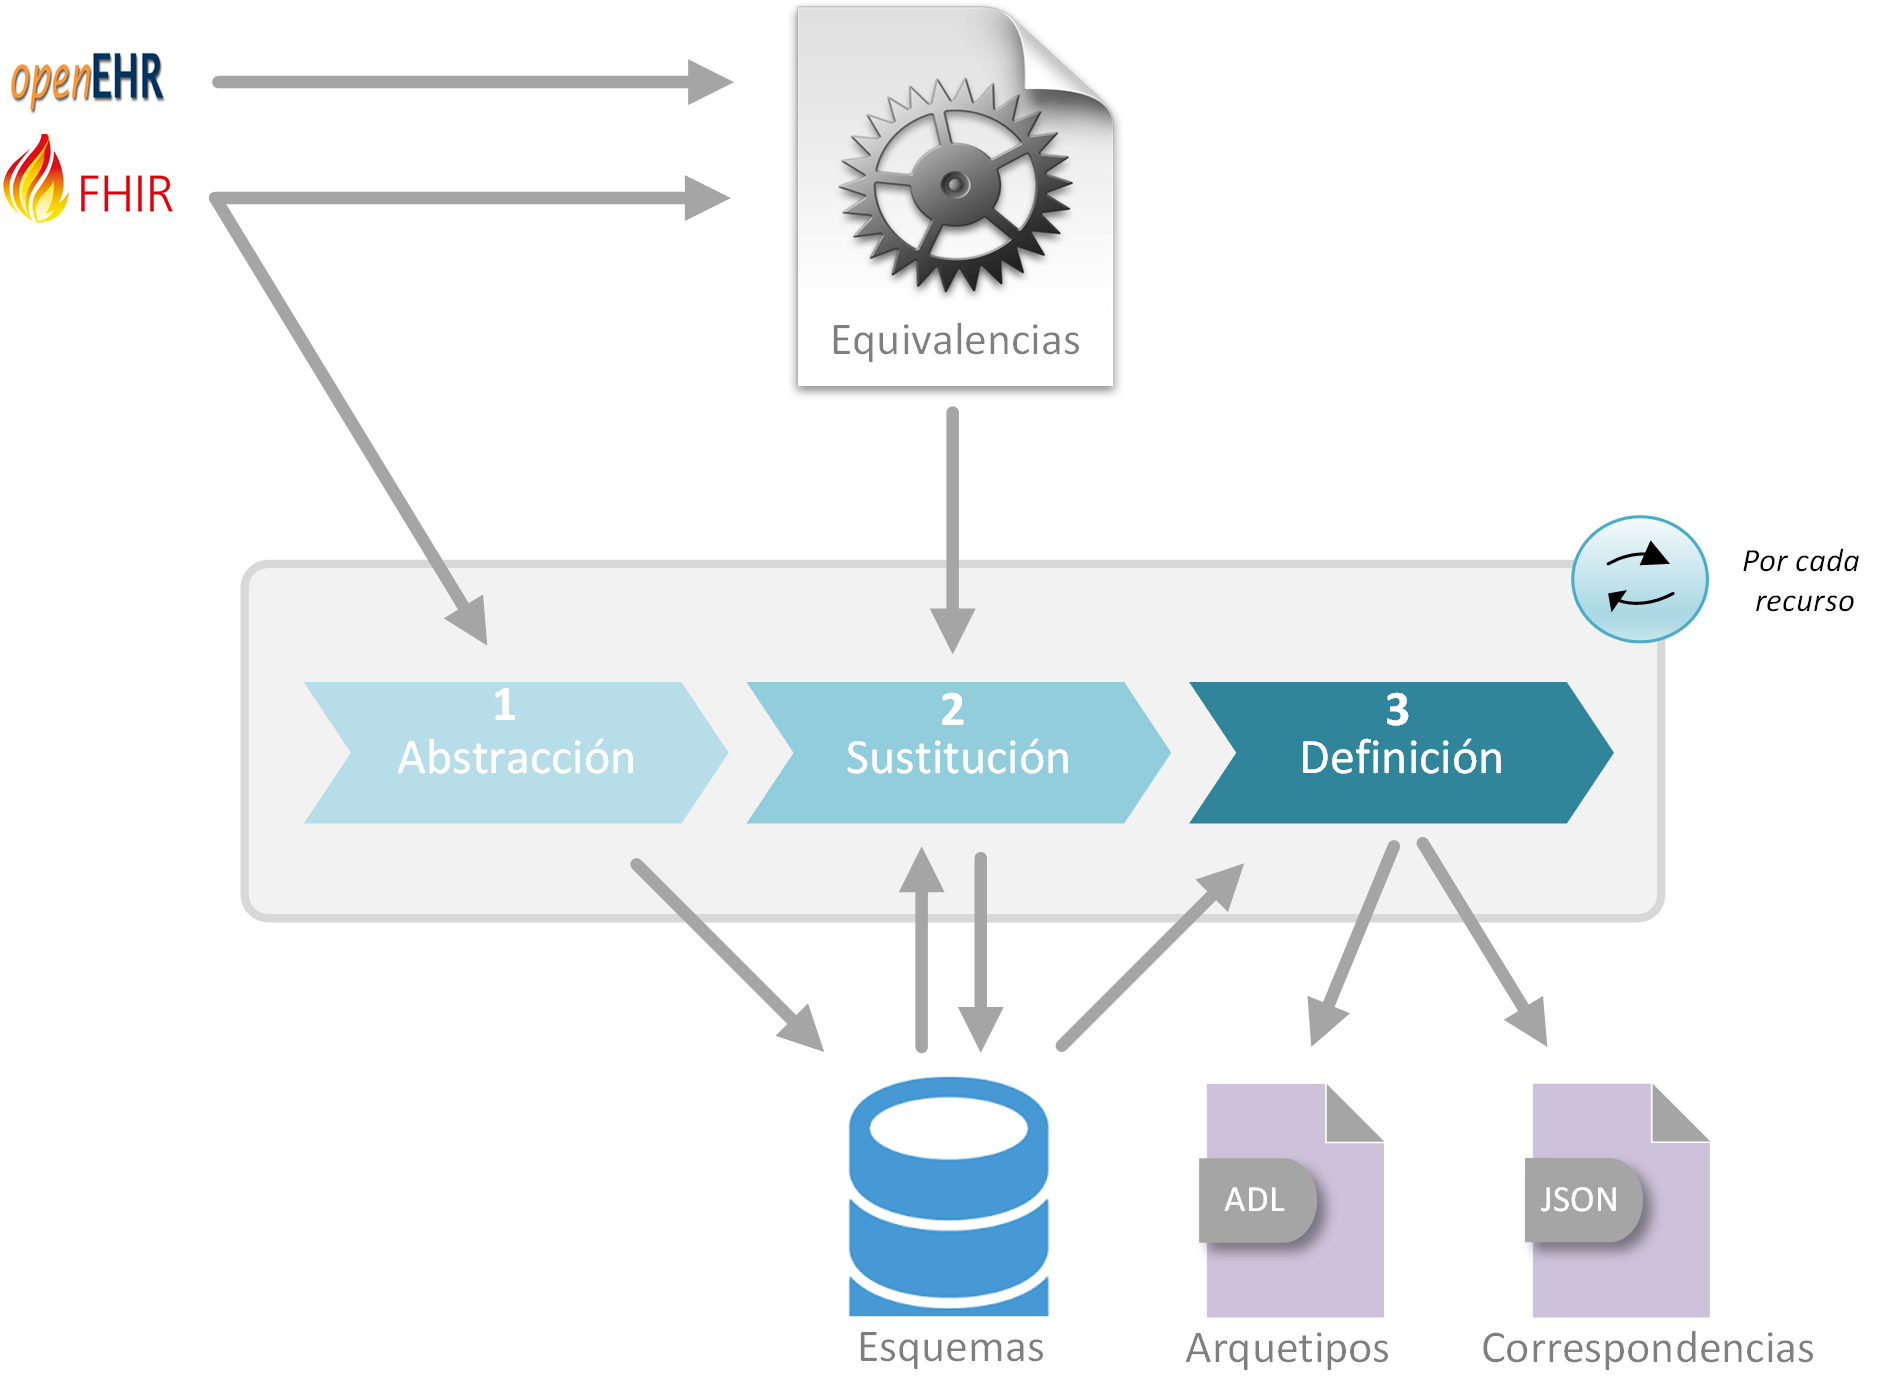
\includegraphics[scale=0.5]{./images/solution.png}
  \caption{Proceso automatizado.}
  \label{fig:solution}
\end{figure}

\subsection{Etapa de abstracción}

El recurso FHIR se modela dentro de un sistema de tipos similar al desarrollado en \cite{Maldonado09}. Cada elemento del recurso FHIR se abstrae por el tipo que describe su estructura. La definición de un tipo es de la forma:

\begin{align*}
T_t:=p_t\{h_t\}
\end{align*}

\noindent
donde \(T_t\) es el nombre del tipo \(t\), \(p_t\) es el predicado que describe los valores soportados por el tipo \(t\) y \(h_t\) es un CML que especifica los elementos hijos que puede tener el tipo \(t\).

La definición del recurso FHIR \(R\) con elementos \(E_1\), \dots , \(E_2\) se abstrae con la definición de tipo como sigue:

\begin{align*}
T_R:=es\_R\{T_{E_1}^{(min_{E_1} \colon max_{E_1})} \dots T_{E_2}^{(min_{E_2} \colon max_{E_2})}\}
\end{align*}

\noindent
donde \(T_{E_1}\) es el tipo que define el elemento \(E_1\), \(min_{E_1}\) y \(max_{E_1}\) son los límites inferior y superior respectivamente de las veces que se permite que el elemento \(E_1\) aparezca en el recurso \(R\). La diferencia con el CML introducido en \cite{Maldonado09} es que en la definición de un tipo no se utilizan las restricciones de longitud por no agregar información adicional a la abstracción de un recurso FHIR.

Para modelar vinculaciones, se extiende el sistema de tipos presentado en \cite{Maldonado09}, agregando definiciones de vinculación. Una definición de vinculación es de la forma:

\begin{align*}
[T_E] := CV
\end{align*}

\noindent
donde \(T_E\) es la definición del tipo del elemento al cual se le vincula el conjunto de valores \(CV\).

Por ejemplo, al considerar el recurso SimplePatient (simplificación del recurso FHIR Patient \cite{FHIRPatient}) que modela un paciente que tiene un solo elemento gender del tipo code \cite{FHIRDataTypes} vinculado al conjunto de valores AdministrativeGender \cite{FHIRAdministrativeGender}, se modela por el conjunto de tipos:

\begin{align*}
&T_{SimplePatient}:= \\
&\qquad es\_SimplePatient\{T_{SimplePatient.gender}^{(0:1)}\} \\
&T_{SimplePatient.gender}:= \\
&\qquad es\_gender\{T_{SimplePatient.gender.code}^{(1:1)}\} \\
&T_{SimplePatient.gender.code}:= \\
&\qquad es\_code\{\epsilon\} \\
&[T_{SimplePatient.gender.code}] := \\
&\qquad URL \footnotemark[1] \\
\end{align*}

\footnotetext[1]{https://www.hl7.org/fhir/valueset-administrative-gender.html}
Un conjunto de tipos que define un recurso FHIR se denomina esquema FHIR en este trabajo.

\subsection{Etapa de sustitución}

El esquema basado en tipos de datos FHIR generado en la etapa previa se transforma en un esquema basado en tipos de datos openEHR. Si se considera las definiciones de un tipo FHIR y de un tipo openEHR:

\begin{align*}
&T_{FHIR}:=p\_FHIR\{h_{FHIR}\} \\
&T_{OPENEHR}:=p\_OPENEHR\{h_{OPENERH}\}
\end{align*}

\noindent
Y existe una equivalencia entre ambos tipos según las condiciones mencionadas en la sección equivalencias entre tipos de datos:

\begin{align*}
&T_{FHIR} = T_{OPENEHR}
\end{align*}

\noindent
Entonces por relación transitiva:

\begin{align*}
p\_FHIR\{h_{FHIR}\} = p\_OPENEHR\{h_{OPENEHR}\}
\end{align*}

\noindent
Por tanto ambas expresiones son intercambiables entre sí y la sustitución es directa. Cada definición de un tipo de dato FHIR se reemplaza por una definición de tipo de dato openEHR equivalente. Cada definición de vinculación sobre un tipo de dato FHIR se sustituye por una definición de vinculación sobre un tipo de dato openEHR equivalente.

Por ejemplo, el esquema FHIR del recurso SimplePatient se transforma al reemplazar la definición del tipo FHIR code por la definición del tipo openEHR DV\_TEXT equivalente en:

\begin{align*}
&T_{SimplePatient}:= \\
&\qquad es\_SimplePatient\{T_{SimplePatient.gender}^{(0:1)}\} \\
&T_{SimplePatient.gender}:= \\
&\qquad es\_gender\{T_{SimplePatient.gender.DV\_TEXT}^{(1:1)}\} \\
&T_{SimplePatient.gender.DV\_TEXT}:= \\
&\qquad es\_DV\_TEXT\{T_{SimplePatient.gender.DV\_TEXT.value}^{(1:1)}\} \\
&T_{SimplePatient.gender.DV\_TEXT.value}:= \\
&\qquad es\_value\{T_{string}^{(1:1)}\} \\
&[T_{SimplePatient.gender.DV\_TEXT.value}] := \\
&\qquad URL \footnotemark[1] \\
&T_{string}:= \\
&\qquad es\_string\{\epsilon\} \\
\end{align*}

Un esquema basado en tipos de datos openEHR se le denomina esquema openEHR en este trabajo. Como se observa, los esquemas FHIR y openEHR de SimplePatient conservan la misma estructura que la definida por el recurso SimplePatient.

\subsection{Etapa de definición}

Según las definiciones de un esquema openEHR, se crea un arquetipo de integración openEHR usando Archetype Definition Language (ADL) \cite{openEHRADL}.

Como identificador del nuevo arquetipo openEHR se usa un nombre de espacio fhir y el nombre del recurso FHIR que el esquema openEHR modela. Por ejemplo, el identificador del arquetipo openEHR del recurso SimplePatient es:

\begin{lstlisting}
fhir::openEHR-EHR-CLUSTER.SimplePatient.v1.0.0
\end{lstlisting}

Para la definición del nuevo arquetipo openEHR, los tipos del esquema openEHR abstraídos de tipos primitivos de FHIR son expresados usando la estructura ELEMENT, y los demás tipos del esquema openEHR son expresados usando la estructura CLUSTER. Ambas estructuras pertenecen al Modelo de Información de Estructuras de Datos de openEHR \cite{openEHRDataStructures}. Por ejemplo, la sección de definición del arquetipo openEHR del recurso SimplePatient usa las clases openEHR CLUSTER y openEHR ELEMENT para los tipos \(T_{SimplePatient}\) y \(T_{SimplePatient.gender}\) respectivamente:

\begin{lstlisting}[mathescape=true]
CLUSTER[id1] $\in$ {
  items $\in$ {
    ELEMENT[id2] occurrences $\in$ {0..1} $\in$ {
      value $\in$ {
        DV_TEXT[id3]
      }
    }
  }
}
\end{lstlisting}

Las definiciones de vinculación se agrega en la sección de vinculación de términos del nuevo arquetipo openEHR. Por ejemplo, la definición de vinculación del tipo \(T_{SimplePatient.gender.DV\_TEXT.value}\) del recurso SimplePatient se transcribe en la sección de vinculación de términos de su arquetipo openEHR equivalente:

\begin{lstlisting}[escapechar=$]
term_bindings = <
  [``fhir"] = <
    [``id3"] = < URL$\footnotemark$ >
  >
>
\end{lstlisting}

\footnotetext{https://www.hl7.org/fhir/valueset-administrative-gender.html}

Los arquetipos openEHR permiten las formaciones de rutas ADL, las cuales sirven para identificar elementos de los arquetipos openEHR \cite{openEHRArchitecture}. En esta etapa, se crea las rutas ADL del nuevo arquetipo openEHR y se relaciona con las rutas de los elementos de su recurso FHIR equivalente. Considerando el recuso de SimplePatient, la relación que se establece es:

\begin{lstlisting}[mathescape=true]
SimplePatient.gender $\Leftrightarrow$ /items[id2]/value[id3]
\end{lstlisting}

    \chapter{Resultados}

\section{Equivalencias entre tipos de datos}

Las equivalencias encontradas entre los tipos de datos FHIR y los tipos de datos openEHR se presentan en el Cuadro \ref{table:equivalents}.

\begin{table}[h]
  \caption{Equivalencias entre tipos de datos}
  \label{table:equivalents}
  \begin{tabular}{l l}
    \hline
    Tipo de dato FHIR &	Tipo de dato openEHR \\
    \hline
    Boolean	& DV\_BOOLEAN \\
    Integer	& DV\_QUANTITY \\
    String	& DV\_TEXT \\
    Decimal	& DV\_QUANTITY \\
    Uri	& DV\_URI \\
    base64Binary	& DV\_PARSABLE \\
    Instant	& DV\_DATE\_TIME \\
    Date	& DV\_DATE \\
    dateTime	& DV\_DATE\_TIME \\
    Time	& DV\_TIME \\
    Code	& DV\_TEXT \\
    Oid	& DV\_URI \\
    id 	& DV\_TEXT \\
    Markdown	& DV\_PARSABLE \\
    unsignedInt	& DV\_QUANTITY \\
    positiveInt	& DV\_QUANTITY \\
    \hline
  \end{tabular}
\end{table}

Cabe mencionar que para todos los tipos de datos FHIR se encuentra su equivalente en openEHR, observándose que ambos estándares comparten los mismos valores de dominio. Los tipos de datos openEHR listados en el Cuadro \ref{table:equivalents}, salvo el tipo DV\_QUANTITY, tienen un atributo value que soporta los valores de sus tipos de datos FHIR equivalentes. El tipo DV\_QUANTITY soporta los valores de sus tipos de datos FHIR equivalentes en su atributo magnitude. Una caso particular es la equivalencia entre el tipo String y el tipo DV\_TEXT. El tipo String puede contener los carácteres Unicode  de tab horizontal, retorno de carro y avance de línea, los cuales no están permitidos en el tipo DV\_TEXT.

Además, se verifica a partir de las especificaciones que las clases de openEHR mantienen sus propósitos.

\section{Arquetipos de Integración}

Las equivalencias entre tipos de datos y el proceso automatizado permiten crear los arquetipos de integración basados en las clases CLUSTER y ELEMENT. Estos arquetipos de integración tienen el propósito principal de ser el punto de entrada de proceso de conversión semántico para importación de datos a sistemas openEHR. La Figura \ref{fig:comparison} muestra de lado a lado un extracto de un arquetipo de integración de paciente creado utilizando el proceso automatizado y el recurso FHIR Paciente del cual se creo.

\begin{figure*}
  \centering
  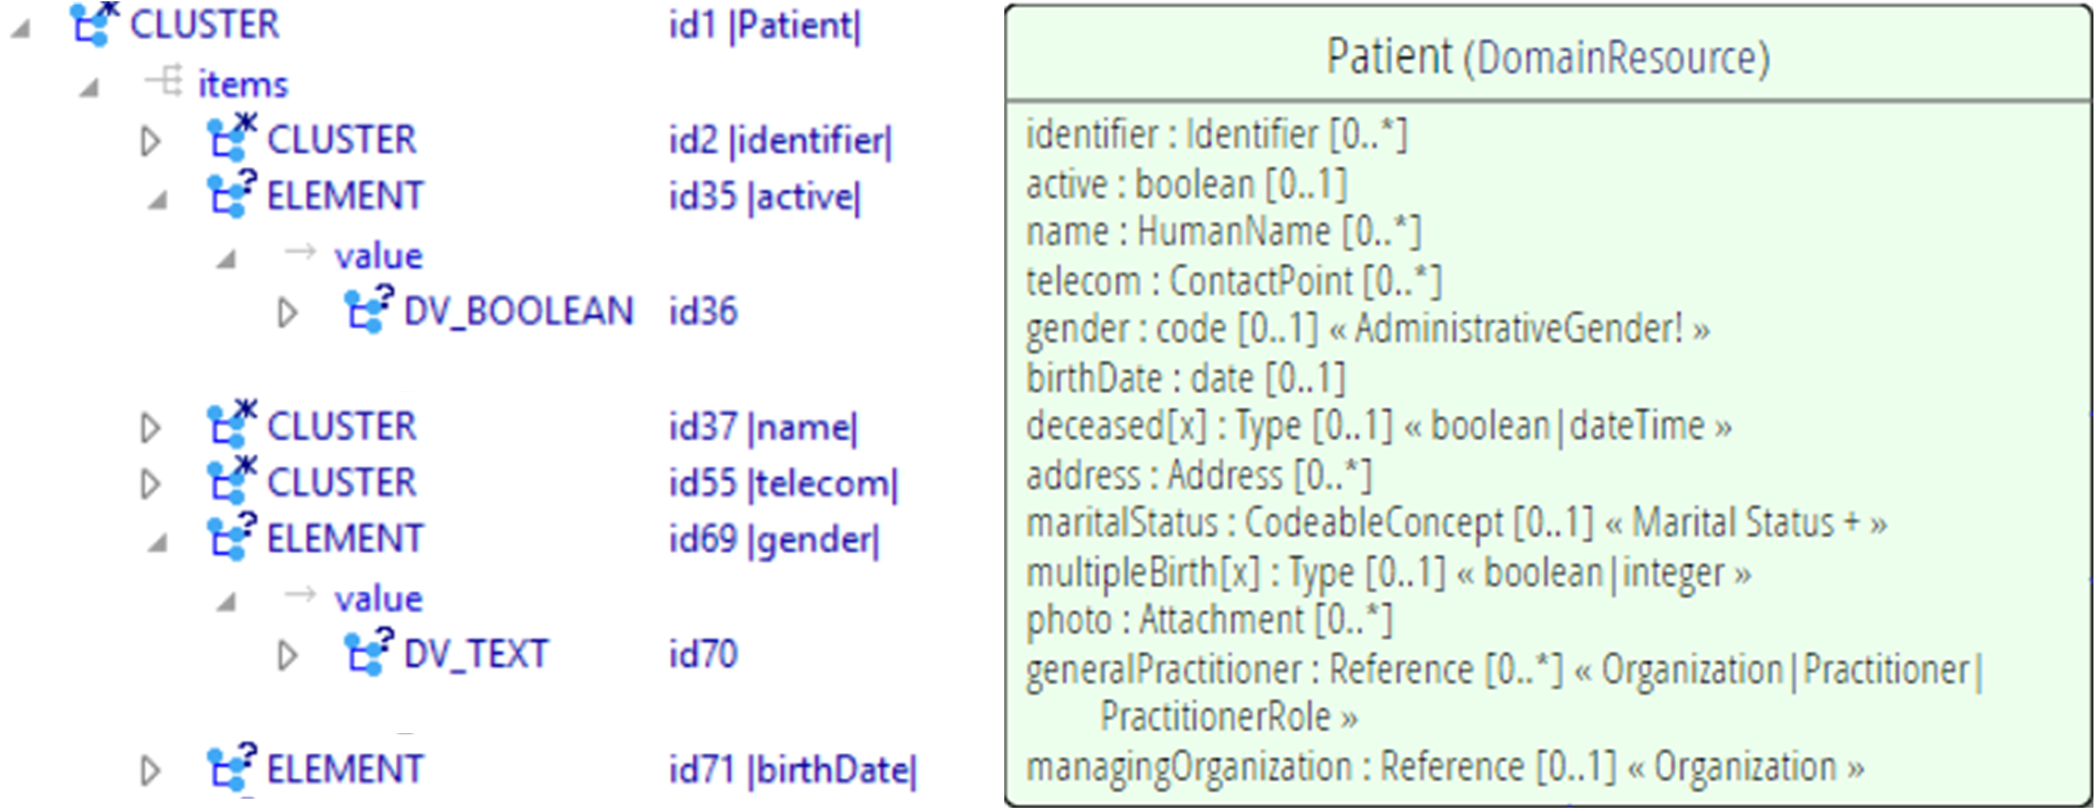
\includegraphics[scale=0.8]{./images/comparison_patient.png}
  \caption{Comparación de un arquetipo de integración de paciente y un recurso de FHIR paciente.}
  \label{fig:comparison}
\end{figure*}

\section{Automatización}

Dentro del atributo snapshot de un recurso FHIR StructureDefinition se encuentra las definiciones de los elementos de un recurso FHR. Un elemento de un recurso FHIR se define en un recurso FHIR ElementDefinition \cite{FHIRElementDefinition}. Tanto los recursos FHIR StructureDefinition y FHIR ElementDefinition tienen representaciones en JSON. Estas representaciones se utiliza en el proceso de automatización para crear un arquetipo openEHR de un recurso FHR de la siguiente forma.

Primero en la etapa de abstracción, el nombre de un recurso FHIR se obtiene del atributo id de un recurso FHIR StructureDefinition. Por cada elemento definido en un recurso FHIR StructureDefinition, se obtiene el nombre del elemento, el tipo del elemento, la cardinalidad mínima y la cardinalidad máxima a partir de los atributos id, type, min y max respectivamente de un recurso FHIR ElementDefinition. Con estos datos se crea una definición de un tipo del elemento con el método descripto más arriba. Una definición de vinculación se crea a partir de un atributo binding de un recurso FHIR ElementDefinition.

Durante la etapa de sustitución, se reemplaza los tipos de datos por sus equivalentes utilizando las equivalencias listadas en el Cuadro \ref{table:equivalents}.

Por último en la etapa de definición, se crea bloques ADL CLUSTER y ELEMENT según explicado más arriba con las siguientes consideraciones. Dado que la clase openEHR DV\_QUANTITY requiere el uso de unidades expresadas en UCUM \cite{UCUM}, se utiliza el valor por defecto de 1 dentro del atributo units para denotar sin unidad. Teniendo en cuenta que la clase openEHR DV\_PARSABLE requiere la especificación del formalismo que utiliza, se emplea los valores base64Binary y Markdown para los tipos FHIR base64Binary y Markdown respectivamente. Un aspecto importante es que definiciones recursivas en recursos FHIR no son soportadas en arquetipos openEHR. Estas definiciones recursivas se limitan a 1 nivel de profundidad en la etapa definición. Una implementación en lenguaje Python de las 3 etapas se encuentra disponible en \cite{PythonImplementation}.

Con el fin de comparar los tiempos de creación manual y automática, se llevó a cabo un experimento en el cual se comparó el tiempo requerido para la creación manual del arquetipo openEHR del recurso SimplePatient presentado en este trabajo  y la creación automática de los arquetipos openEHR de los recursos FHIR categorizados como individuos. Para la creación manual se utilizó el editor ADL WORKbench \cite{ADLWORKbench}. Para la creación automática se utilizó el proceso de la Figura \ref{fig:solution} implementado en el lenguaje Python \cite{PythonImplementation}. Los resultados del experimento mostraron que la creación automática de arquetipos openEHR de todos los recursos categorizados como individuos (6 recursos) tomó en promedio 281.53 ms frente a los 79.5 segundos que tomó en promedio la creación manual de la definición del recurso SimplePatient.

    \chapter{Conclusiones}

Intercambiar datos es uno de los requisitos más básicos que openEHR busca satisfacer. Importar y exportar datos por medio de interfaces FHIR sobre repositorios openEHR requiere una conversión de datos. Técnicamente, exiten 2 temas a resolver que son la equivalencia a nivel de estructura y la compatibilidad a nivel de tipo de dato.

El trabajo presentado resuelve la equivalencia estructural creando arquetipos de integración similares a lo expuesto en \cite{openEHRArchitecture}. Estos arquetipos creados se caracterizan por:

\begin{enumerate}
  \item estar basados en las clases CLUSTER y ELEMENT;
  \item estar diseñados para copiar la estructura de datos de recursos FHIR existentes;
  \item existe un arquetipo de integración por recurso FHIR compartido.
\end{enumerate}

Como las estructuras de estos arquetipos de integración son idénticas a las estructuras de los recursos FHIR que se utilizan para intercambiar datos, se puede utilizar las rutas ADL de los arquetipos de integración y las rutas de los elementos de los recusos para establecer reglas de conversión de datos. Estas reglas de conversión pueden usarse en programas de transformación basados en XQuery para convertir instancias de recursos FHIR a instancias de arquetipos de integración openEHR y viceversa. Estos arquetipos de integración pueden ser utilizados por software openEHR o bien mapeados a arquetipos existentes utilizando herramientas como LinkEHR-Ed \cite{Maldonado09}. Este mapeo queda como trabajo futuro y forma parte de la estrategia de integración basada en arquetipos explicada en \cite{openEHRIntegration}.

Una ventaja de la integración basada en arquetipos es que el diseño de los arquetipos de integración lo hace TI u otro personal técnico que esté familiarizado con las estructuras de los datos entrantes, sin involucramiento de los especialistas de dominio. Esto es importante porque delega la responsabilidad de integración de sistemas a personal de TI, mientras mantiene el diseño de los demás arquetipos a cargo de los especialistas de dominio.

En esta estrategia de integración existe la desventaja de tener que crear arquetipos de integración en vez de utilizar directamente los arquetipos disponibles en librerías. Sin embargo, este problema puede solucionarse realizando transformaciones directas entre arquetipos de integración y arquetipos diseñados en librerías. El usar un mismo nombre de espacio fhir para los arquetipos de integración servirá para distinguir estos arquetipos que representan recursos FHIR.

Un problema a resolver es la definición recursiva de recursos FHIR y que en arquetipos openEHR no está permitida. Una forma de resolver es limitando la profundidad de recursividad. Otras formas de solución requieren más trabajo futuro.

De forma a resolver la compatibilidad entre tipos de datos FHIR y openEHR, se propuso una definición de equivalencia con 2 condiciones. La primera condición garantiza que todo dato FHIR puede ser convertido en un dato openEHR. La segunda condición asegura que los datos convertidos puedan ser procesados correctamente.

Una forma de solventar el caso particular de la equivalencia entre el tipo String y el tipo DV\_TEXT es que en la conversión de datos de estos caracteres no impresos se sustituya por su codificación en Unicode para que se pueda almacenar como texto dentro del tipo DV\_TEXT y cuando se recuperen se vuelvan a convertir a su valor original. De esta forma se garantiza que no habrá pérdida de información.

Medicina es un dominio cambiante. Por lo tanto, proveer un proceso de creación automática de arquetipos de integración que ahorre tiempo y reduzca errores es de gran utilidad para el personal técnico. El experimento realizado mostró una reducción significativa en el tiempo de creación usando el proceso automatizado.

En conclusión, las equivalencias de tipos y el proceso automatizado ayuda a que se pueda convertir y procesar correctamente los datos de instancias de recursos FHIR en instancias de arquetipos de integración openEHR, siendo un siguiente paso verificar la posibilidad de crear recursos FHIR de arquetipos openEHR utilizando las equivalencias presentadas y el proceso propuesto en este trabajo.

 % \backmatter
 %\bibliographystyle{abbrv}
  \bibliographystyle{elsarticle-num}
  \bibliography{referencias}

\end{document}
